\section{Our Approach}
Our approach exploits structural information like \FB \CVT tables to  automatically annotate event mentions\footnote{An event mention is a
phrase or sentence within which an event is described, including its type and arguments.} in order to generate training data to learn an
event extractor. Such an approach is known as Distant Supervision (\DS)\FIXME{~\cite{}}. Essentially, we use the knowledge extracted from a
known knowledge base to label sentences from another dataset to generate training data.


We use the arguments of a \CVT table entry to infer what event a sentence is likely to express. A \CVT table entry can have multiple
arguments but not all of the arguments are useful in annotation. For example, the \texttt{divisions\_formed} argument in
Figure~\ref{fig:example} (b) is not as important as the other three arguments when determining if a sentence expresses a
\texttt{business.acquisition} event. Therefore, our first step is to identify the key arguments from a \CVT table entry. A key argument is
an argument that plays an important role in one event, which helps to distinguish with other events. If a sentence contains all key
arguments of an entry in an event table (e.g. a \CVT table), it is likely to express the event expressed by the table entry. If a sentence
is labelled as an event mention of a \CVT event, we also record the words or phrases that match the entry’s properties as the involved
arguments, with the roles specified by their corresponding property names. For instance, sentence S1 shown in Figure~\ref{fig:example} (a)
is a mention of \texttt{business.acquisition} type, its involved arguments are ``Remedy Corp", ``BMC Software", and ``2004", and the roles
of the three arguments are \texttt{company\_acquired}, \texttt{acquiring\_company} and \texttt{date} respectively.

\subsection{Determining Key Arguments}
We use the following formula to calculate the importance value, $I_{cvt, arg}$, of an argument \emph{arg} (e.g., date) to its event type
\emph{cvt} (e.g., \texttt{business.acquisition}):

\begin{equation}
	I_{cvt, arg} = log \frac{count(cvt, arg)}{count(cvt) \times count(arg)}
\end{equation}


where $count(cvt)$ is the number of instances of type $cvt$ within a \CVT table, $count(arg)$ is the number of times $arg$ appearing in all
\CVT types within a \CVT table, and $count(cvt, arg)$ is the number of $cvt$ instances that contain $arg$ across all \CVT tables.


Our strategy for selecting key arguments of a given event type is described as follows. We first calculate the important value of each
argument. Next, we sort the arguments according to their importance values in descending order, so that arguments with the higher
importance values will appear on the top of the list. We then consider arguments on the top half of the list as key arguments. Furthermore,
we find that time-related arguments are useful in determining the event type, so we always include time-related arguments (such as date) in
the key argument set. Using this strategy, the first three argument of the CVT entry are considered to be key arguments for event type
\texttt{business.acquisition}.


\subsection{Justification of Key Argument Selection Strategy}
We use three example sentences from the Wiki text dataset to justify our key argument selection strategy. The three sentences are:

\begin{quote}
\textbf{S2}: \underline{\emph{Microsoft}} spent \$6.3 billion buying online display advertising company \underline{\emph{aQuantive}} in
\underline{\emph{2007}}.
\end{quote}
\begin{quote}
\textbf{S3}: Microsoft hopes aQuantive's Brian McAndrews can outfox Google.
\end{quote}
\begin{quote}
\textbf{S4}: On April 29th, Elizabeth II and Prince Philip witnessed the marriage of Prince William.
\end{quote}
\begin{figure}
\centering
	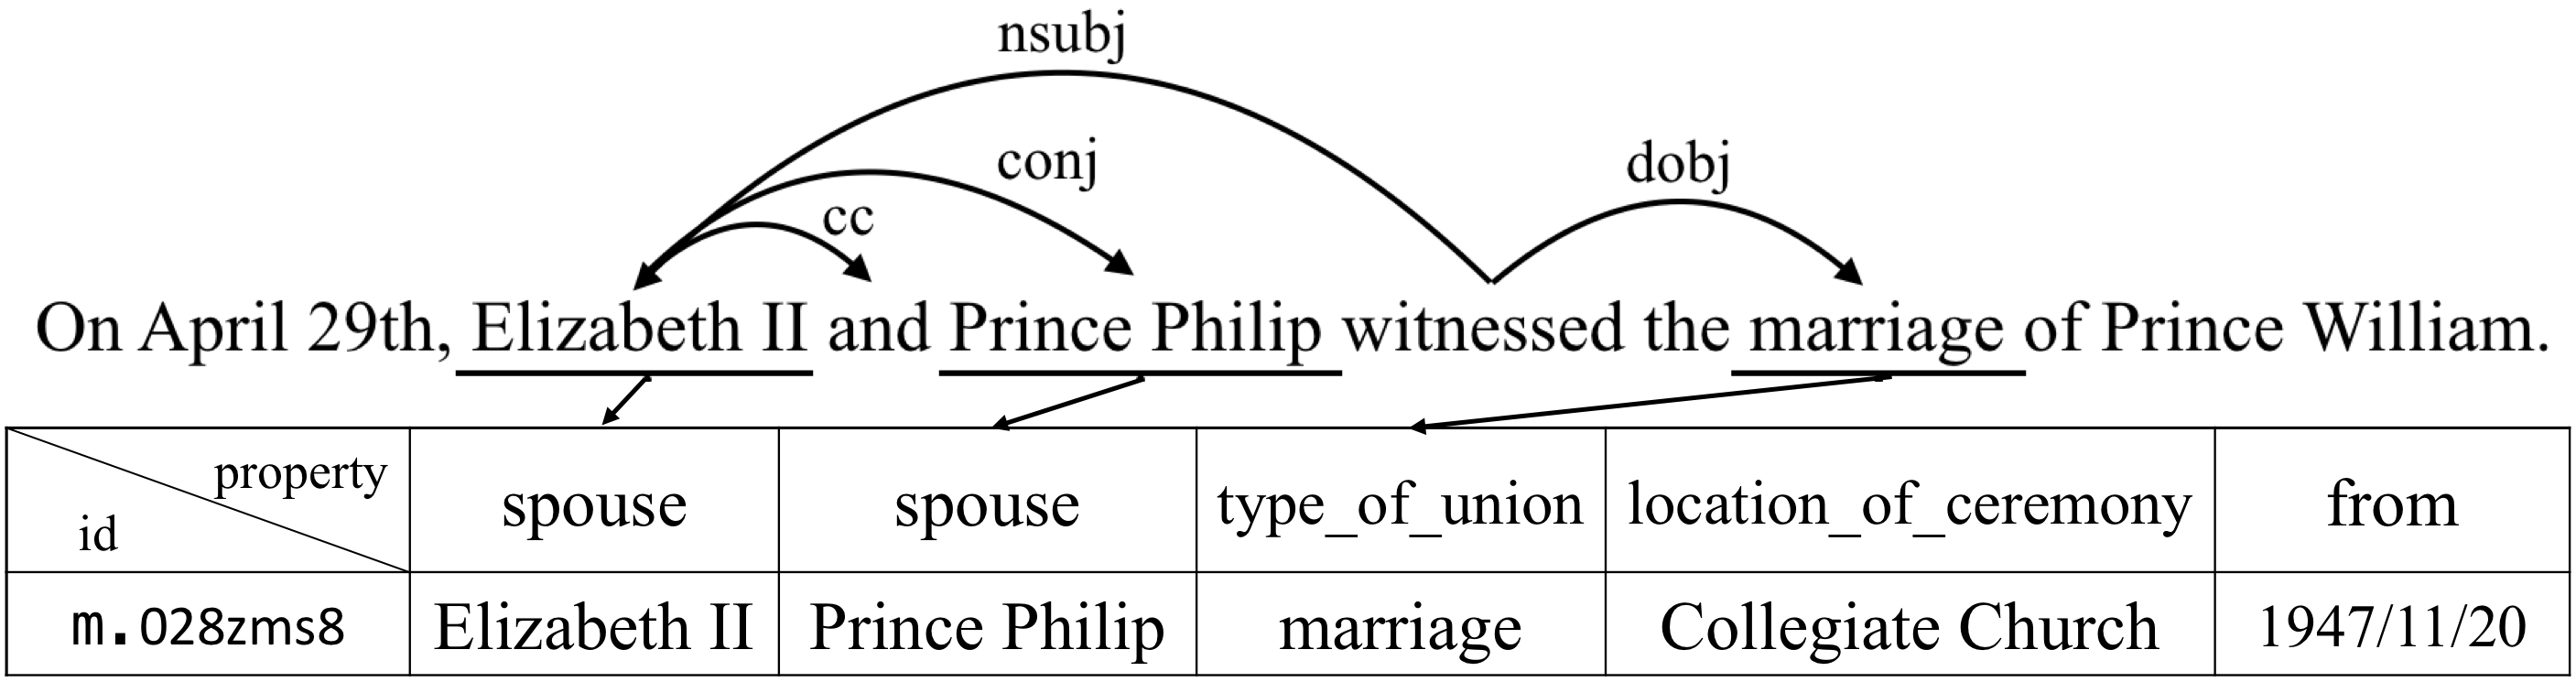
\includegraphics[width=.48\textwidth]{figure2.png}
	\caption{The dependency tree of S4, which partially matches an entry of \emph{people.marriage}. \label{fig:2}}
\end{figure}
We regard a sentence as \emph{positive} when it mentions the occurrence of an event, or  \emph{negative} otherwise. For example, S1 in
Figure~\ref {fig:example} (a) and S2 (with its arguments in italics and underlined) are positive examples, while S3 and S4 are negative.


Intuitively, two arguments involved in the same event mention are likely to be closer within the syntactic structure.  In
Figure~\ref{fig:2}, both \emph{Prince Philip} and \emph{marriage} can be matched as key arguments in a \textit{people.marriage} entry, but
are far from each other on the dependency parse tree, thus S4 should be labelled as negative.
